\mychapter{1}{Introduction}

In this robotics class, we consider the task of making a person hold his/her Raspberry Pi in front of a laptop's webcam.  The Raspberry Pi, equipped with its sense hat,  allows to display a single red dot on its LED matrix so that the webcam can monitor it. The goal of this project is to ensure that the red dot always remains as close as possible to the center of the webcam's captured image. This must particularly hold if the person shakes, moves, or rotates the Raspberry Pi in front of the webcam. If the Raspberry Pi's LED matrix is placed too far from the webcam's image center, the red dot should be placed as close as possible to the latter.

If we were to solve this problem manually, we would need to have access to the Raspberry Pi's accelerometer and gyroscope to determine the speed and the direction of the motion of the red dot on the LED matrix. This would require us to use a reference frame for which the origin would be the center of the webcam's image. Access to acceleration and gyroscopic data would allow to construct a velocity vector anchored at the red dot and pointing towards the origin of this reference frame. Doing so would enable us to undo the person's motions and therefore stabilize the red dot at the center of the image. Although this approach seems technically feasible, its implementation is not straightforward. 

In this course, we intend to use Reinforcement Learning (RL) as a "last-resort" solution to overcome the complexity of the previous approach. Our goal is thus to produce a \textit{policy} that allows to move the red dot on the Raspberry Pi's LED matrix so as to be as close as possible to the center of the image. In order to achieve this goal, we will need the following components:

\begin{itemize}
	\item A Raspberry Pi with a mounted sense hat (comprises the LED matrix);
	\item A laptop with a front webcam;
	\item A Reinforcement Learning agent.
\end{itemize}

In the following sections, we start by explaining how the Raspberry Pi can be set up to communicate with the laptop about the red dot's position on the webcam image.  We also describe how the red dot's position can be retrieved from the raw image using image processing techniques. The last section of this chapter investigates the set up of the RL agent and its corresponding environment.

\section{Configuration of the Raspberry Pi}

In order for the RL agent to decide how to move the red dot on the Raspberry Pi 's LED matrix, the agent must have access to acceleration and gyroscopic data of the Pi. In return, the Pi must have access to the decision of the agent, given this data, in order to re-center the red dot. The actions of the agent are (1) \textit{Move North}, (2) \textit{Move South}, (3) \textit{Move West}, (4) \textit{Move East} and (5) \textit{Stay}.  Both entities thus communicate according to the scheme of figure \ref{communication}.

\begin{figure}

\centering

\begin{tikzpicture}[
squarednode/.style={rectangle, draw=black!60, fill=black!5, very thick, minimum size=5mm},
]
%Nodes
\node[squarednode]      (agent)                             {RL Agent};
\node[squarednode]      (rasp)   [right=of agent] {Raspberry Pi};

%Lines
\draw[->] (agent.north) to [out=90,in=90]     node[midway,  above]   {Action: North, South, West, East, Stay}  (rasp.north) ;
\draw[->] (rasp.south)   to [out=-90,in=-90]  node[midway, below]    {Acceleration $\&$ Gyroscope}             (agent.south);

\end{tikzpicture}

\caption{Communication between the Raspberry Pi and the RL agent. The Pi sends its acceleration and gyroscopic data over to the agent which decides what action to take in order to re-center the red dot on the webcam image.} 
\label{communication}
\end{figure}

To ensure a communication between both entities, we implement a Python socket server on both sides over the same wifi network. On the Pi, we create a python socket server using code inspired from the project description. Section \ref{server_code} of the Appendix illustrates this process. Apart from the functions for sending and receiving objects from/to the server, a Sensehat instance is created, along with a Raspberry instance. The Sensehat object is responsible for

\begin{enumerate}
\item displaying the LED light through its \texttt{\detokenize{set_pixel()}} method;
\item sampling acceleration data through its  \texttt{\detokenize{get_accelerometer_raw()}} method;
\item sampling gyroscopic data through its  \texttt{\detokenize{get_gyroscope_raw()}} method.
\end{enumerate}

The Raspberry instance on the other hand wraps the Sensehat instance into a class which has these acceleration and orientation measures as properties.  The code of section \ref{rasp_code} illustrates this process. In order to close the loop of figure \ref{communication}, the Raspberry instance needs a function that translates the action prescribed by the agent into a visible result. This is exactly the purpose of the  \texttt{\detokenize{move_led()}} function of this class, which executes all five actions described above.

\section{Webcam image processing}

For the agent to prescribe actions to the Pi as shown on figure \ref{communication}, it must be able to detect the position of the red dot on the LED matrix. It is clear that the reliable nature of the detection of this red dot is crucial for the project's success. Indeed, if this detection were to fail or to produce imprecise results, it would inevitably affect the learning of the agent. For our agent to learn properly, it is crucial to develop a technique that extracts the position of the red dot from the webcam's image with small influence of the surrounding light. We will use the OpenCV library to perform this task. A first step toward this task is to get familiar with standard image processing techniques proposed by OpenCV. One important feature is the use of \textit{masks} to process an image. Such masks basically filter out specific regions of an HSV image so as to produce an image with enhanced contrasts for certain objects. In our case, we wish to extract the regions of the image with bright red colours. An important drawback of the Pi's LED matrix is that the red light seen by us humans is, in fact, not predominantly red. The emitted light is indeed shifted towards ultraviolet wavelengths, which makes its detection hard, especially in when placed in an environment with daily light as the one of figure \ref{no_filter}. Thus before implementing a complete filtering of the image's red components, I decided to get a feeling of how the filtered image reacts to cuts in \textit{h}, \textit{s} and \textit{v} values. I therefore used the script of section \ref{calibrate} to produce cursors that filter the image in real time. Figure \ref{filter} shows the result of applying $h \in [0, 45] $,  $s \in [0, 255]$ and $v \in [150, 255]$. After playing around with those cursors, I came up with the following conclusions:

\begin{itemize}
	\item The image is very sensitive to  \texttt{\detokenize{s_min}} (keep it at $0$);
	\item Proper red filtering can only be done using two intervals of \texttt{\detokenize{h}} around $0$ and $180$;
	\item Only very high brightness allows to discriminate daily light from the Pi's LED light (keep \texttt{\detokenize{v}} between $217$ and $255$)
\end{itemize}

\begin{figure}[H]

  \begin{minipage}[b]{0.45\linewidth}
   \centering
   \includegraphics[width=6.5cm,height=5cm]{Images/calibrate.png}
   \caption{Image processing using OpenCV with $h \in [0, 45] $,  $s \in [0, 255]$ and $v \in [150, 255]$.}
   \label{filter}
  \end{minipage}
\hfill
  \begin{minipage}[b]{0.45\linewidth}
   \centering
   \includegraphics[width=6.5cm,height=5cm]{Images/calibrate2.png}
   \caption{Original image with no filter.}
   \label{no_filter}
  \end{minipage}
\end{figure}

This first trial with the OpenCV library helped me produce a full preprocessing pipeline of the original webcam image. The function \texttt{\detokenize{filter_image()}} of section \ref{processing} implements this process:

\begin{enumerate}
	\item Apply a first lower and upper mask using $h \in [0, 10] \cup [90,179] $,  $s \in [0, 255] \cup [0,255]$ and $v \in [217, 255] \cup [230,255]$;
	\item Re-apply a red filter using $h \in [10, 180] $,  $s \in [0, 150]$ and $v \in [0, 255]$;
	\item Filter the image using a binary threshold set on $150$ pixel value.
\end{enumerate}

The careful reader will however have noticed that the red dot itself was not captured by these processing techniques. Instead the \textit{contour} of the LED cell was highlighted (see final figure \ref{opencv:threshold}). The idea of capturing the contour of the dot rather than its center was forced by the fact that the LED light seemed to somehow "burn" the built-in camera of my Macbook, making its center invisible after applying the first red filter.  In addition, applying the \texttt{\detokenize{compute_red_dot()}} function of section \ref{processing} allows to get back our red dot since OpenCV's \texttt{\detokenize{connectedComponentsWithStats()}} function computes the position of the biggest visible area. 

\begin{figure}[H]

  \begin{minipage}[b]{0.45\linewidth}
   \centering
   \includegraphics[width=7cm,height=5cm]{Images/original.png}
   \caption{Original webcam image with the computed red dot position in red and image center in purple.}
   \label{opencv:original}
  \end{minipage}
\hfill
  \begin{minipage}[b]{0.45\linewidth}
   \centering
   \includegraphics[width=7cm,height=5cm]{Images/red_filter.png}
   \caption{Result of the application of the first red filter.}
   \label{opencv:red_filter}
  \end{minipage}
\end{figure}

\begin{figure}[H]

  \begin{minipage}[b]{0.45\linewidth}
   \centering
   \includegraphics[width=7cm,height=5cm]{Images/additional_red_filter.png}
   \caption{Webcam image after re-applying a red dominance filter on the image of figure \ref{opencv:red_filter}.}
   \label{opencv:add_filter}
  \end{minipage}
\hfill
  \begin{minipage}[b]{0.45\linewidth}
   \centering
   \includegraphics[width=7cm,height=5cm]{Images/threshold.png}
   \caption{Final thresholded image that displays the red dot in gray scale.}
   \label{opencv:threshold}
  \end{minipage}
\end{figure}

Instead of computing the center of a rectangle, it simply computes the center of an arc which gives approximately the same result. Doing so revealed the capturing of the dot's contour to be surprisingly robust against changes in environmental light. The agent therefore benefits from a processing routine \texttt{\detokenize{get_red_dot()}} that allows it to have a reliable access to the red dot's position on the webcam image.

\section{Set up of the environment}

The next step of the project consists in creating an environment for the RL agent. For this we will use the OpenAI Gym library. The requirements on our custom environment are the following:

\begin{itemize}
	\item Inherit from the gym's environment class;
	\item Define an action and observation space;
	\item Implement the \texttt{\detokenize{step()}} and \texttt{\detokenize{reset()}} methods.
\end{itemize}

The code for this new environment is given in section \ref{environment}. Since there are 5 different actions to be considered, the action space is a 5-dimensional discrete set. The observation space on the other hand is made of the acceleration $(a_x, a_y, a_z)$ and gyroscopic $(g_x, g_y, g_z)$ data as well as the position of the red dot $(x,y)$ computed by the \texttt{\detokenize{get_red_dot()}} routine, which results in a 8-dimensional box. It is important to note that both the frame of the webcam image and the position of the red dot on it are declared as properties of the \texttt{\detokenize{RaspEnv}} class. When called during training, the \texttt{\detokenize{get_red_dot()}} routine will update the class' frame via OpenCV's \texttt{\detokenize{VideoCapture}}'s instance and set the red dot to the detected position. The square setter therefore allows to make sure the agent is trainable when updating the dot's position by making sure it is not set to \texttt{\detokenize{None}} (i.e., the red dot is lost on the image).
The environment's \texttt{\detokenize{step()}} function is called iteratively during training and therefore does not need any additional internal or external \texttt{\detokenize{for}} loop. It simply sends the action prescribed by the agent, waits 0.2 seconds for the Pi to execute it before constructing it's observation based on the acceleration and gyroscope sent by the Pi and the new (normalized) dot position. The normalization is done using the relative distance to the image center. Let us note that if the new dot position is \texttt{\detokenize{None}}, the environment is being reset before resuming training. Also note that the red dot is assigned to a new random position every time the environment is being reset.
A last key component of our environment is the reward associated to each state-action pair. Following the update of the red dot's position, we used the normalized distance to the image center to compute the associated reward. As will be highlighted in the results, we used the exponential of the euclidean distance as a reward measure, the graph of which is displayed on figure \ref{reward_dist}.

\begin{equation}
	r(x,y) = 1 - e^{\sqrt{x^2 + y^2}},
	\label{gaussian_reward}
\end{equation}

where $x$ and $y$ are the normalized coordinates with respect to the image center.

\begin{figure}[H]
	\centering
	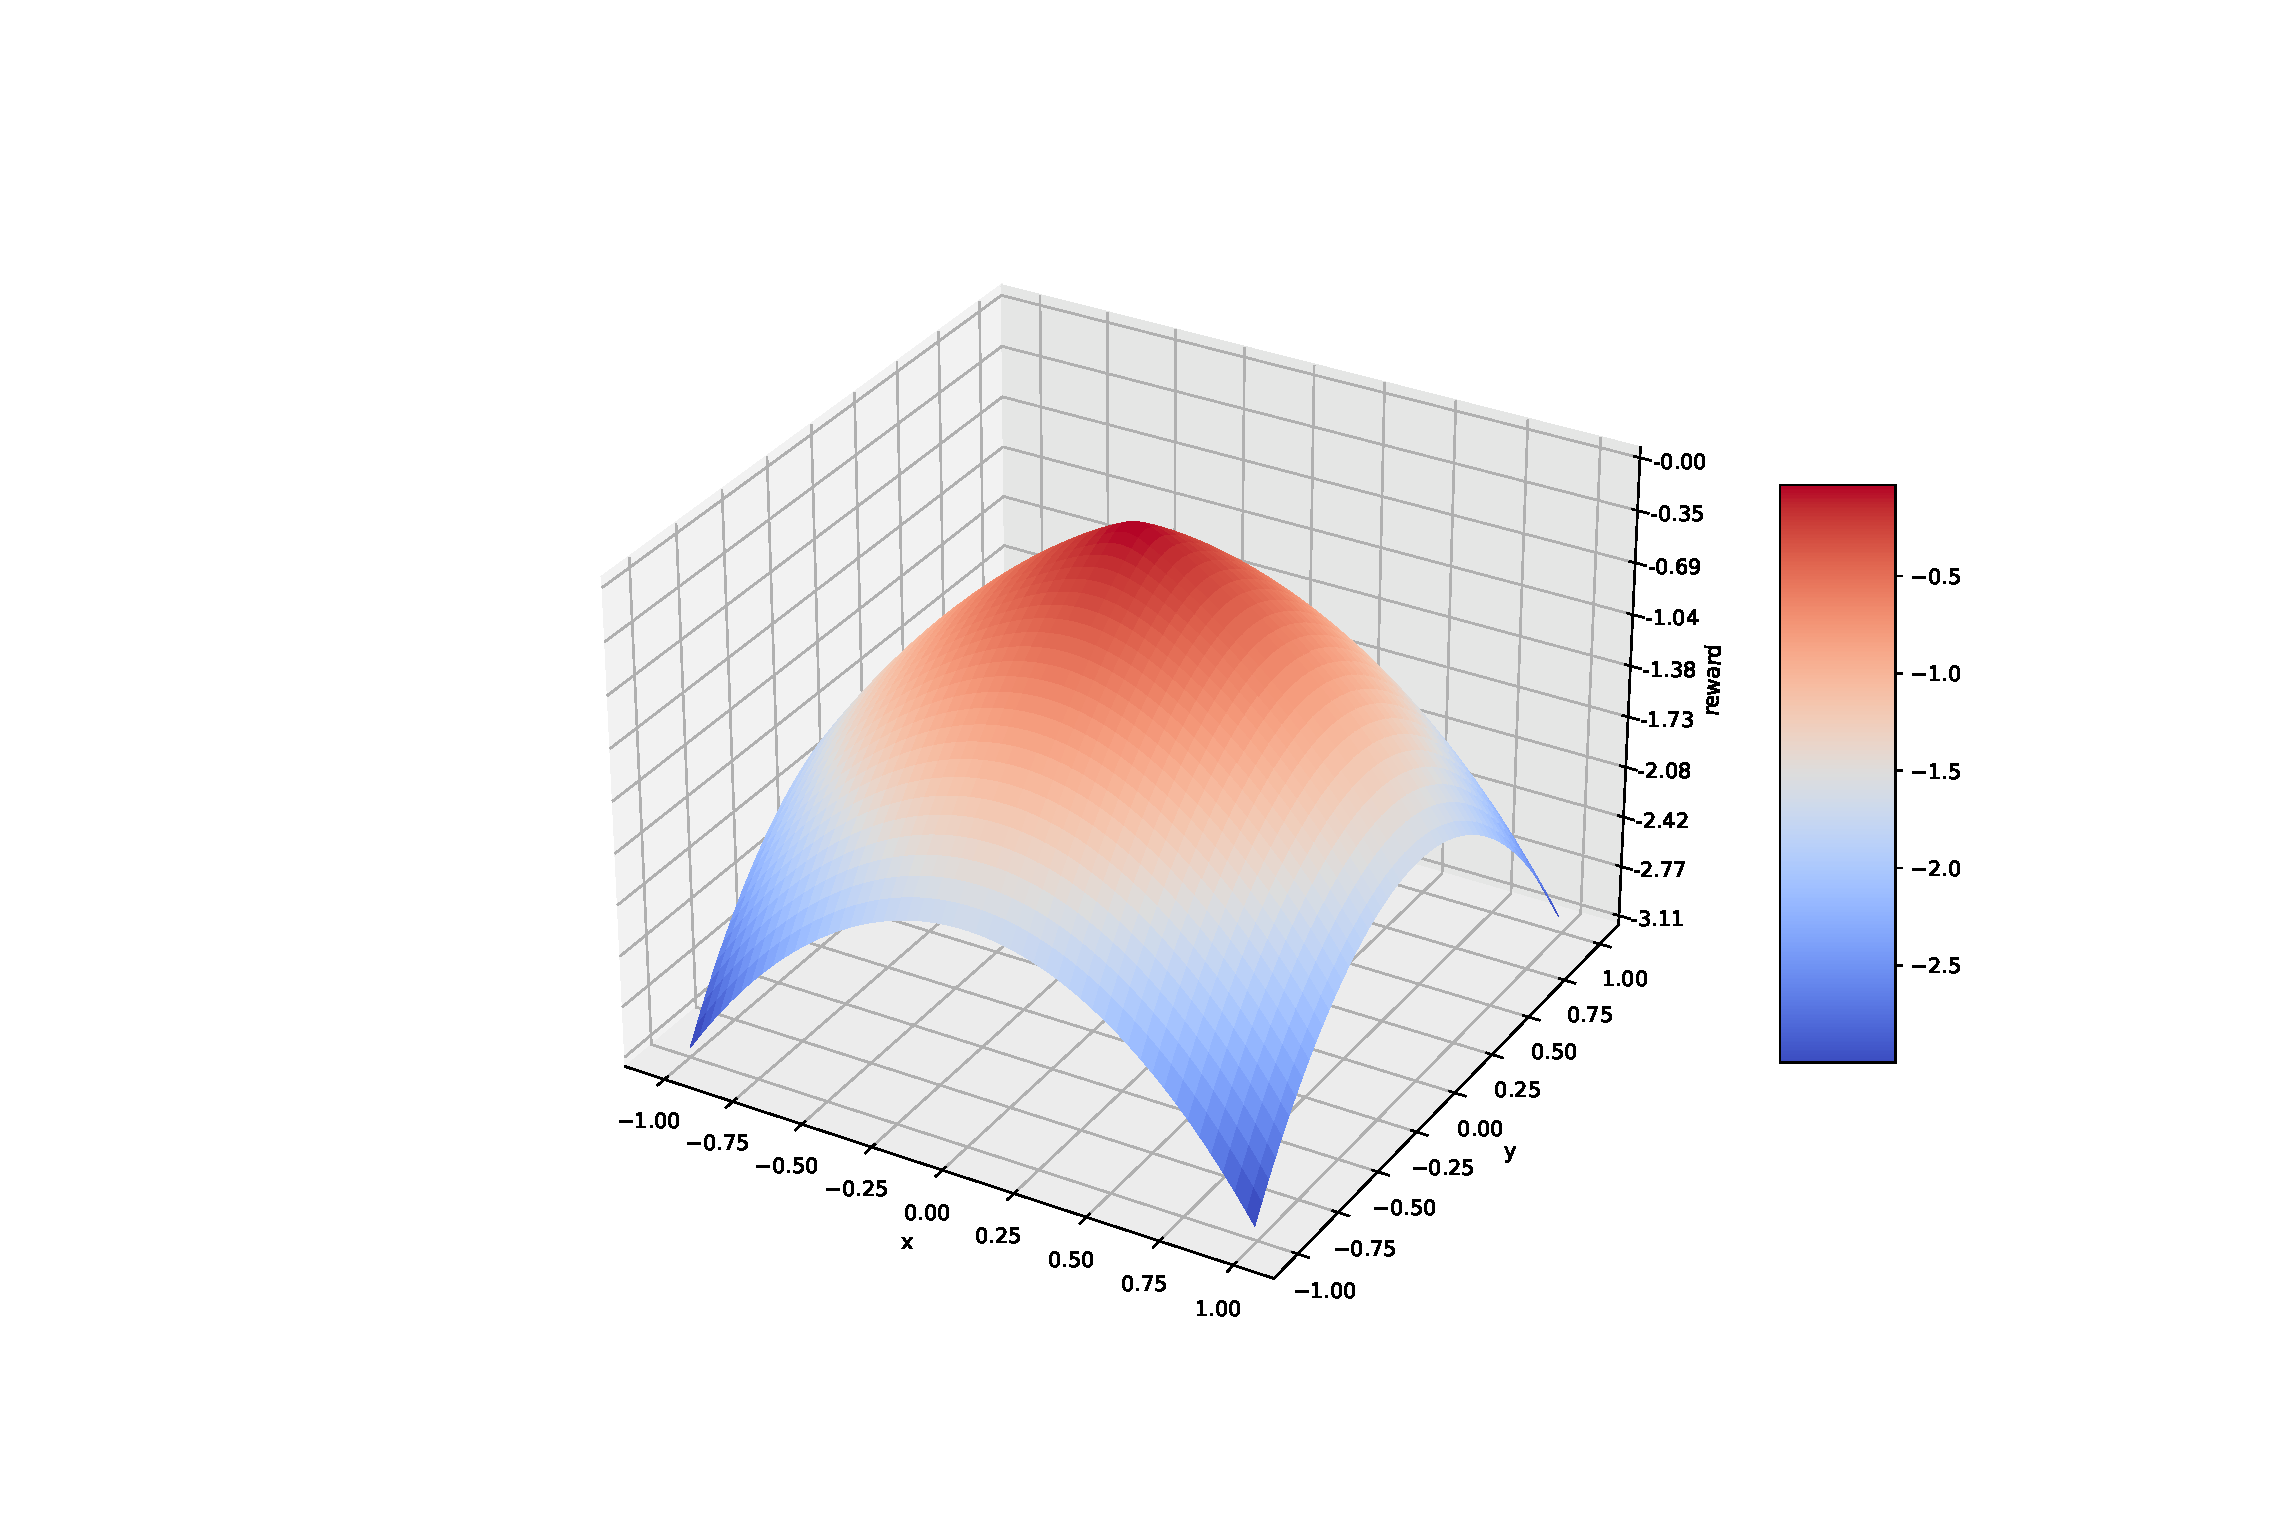
\includegraphics[scale=0.35]{Images/reward.eps}
	\caption{Reward distribution. The exponential of the euclidean distance is aimed to further penalize large distances to the image center.}
	\label{reward_dist}
\end{figure}

The project set up is now complete; our agent benefits from a gym environment in which it can learn. It is also able to detect the red LED light on the Pi's LED matrix and communicate with it. To make our agent learns how to maintain the red dot centered on the webcam image, we need to choose a dedicated RL algorithm and train it, which is the purpose of the next chapter.

\mychapter{2}{Results}

In order to train our agent in the environment we just set up, we simply need to choose a RL algorithm and train it in this environment for a predefined number of time steps. A key feature of this project is the ability of the user to stop training at a certain moment and to be able to resume training at the stage where he/she left. This is done using checkpoint callbacks every 1000 time steps. Each run therefore results in a partially trained agent stored in the "model checkpoints" folder of the code. At the beginning of each run, the agent's \texttt{\detokenize{train()}} function will try to load the most recent model (\texttt{\detokenize{load_model()}}) and if it does not find any, it will simply create a new one (\texttt{\detokenize{create_model()}}). Also note that the tensorboard logs are stored in a predefined path in order to monitor the training of the agent during and after training.  The code relative to the agent is given in section \ref{agent}. In the following sections, we will analyze and compare the performances of the actor-critic PPO2 algorithm from stable-baselines and the Deep-Q network approach.

\section{PPO2}

The first algorithm I investigated is the actor-critic PPO2 algorithm of the stable-baselines library. Although PPO2 has a few hyperparameters one could tune, I decided to go with the default parameters for this first agent. Besides,  two important aspects of this first run significantly affected the learning process:

\begin{enumerate}
	\item The observation space has large lower and upper bounds;
	\item The negative normalized euclidean distance between the red dot's position and the image center is used as a reward.
\end{enumerate}

Doing so produces a reward that potentially ranges from $-\sqrt{2}$ (location of one corner) to $0$ (image center). In the first trial, the Raspberry Pi was maintained in the same position in order to verify that the agent is able to place the red dot at the desired location without any perturbation of the Pi's position and orientation. In these settings, the agent experienced a first drop in discounted reward before starting to learn after approximatively $6000$ time steps.  Figure \ref{reward_dist} indeed shows this trend. The sudden drops around $10000$ and $27000$ time steps are due to the resuming of training. The signal indeed drops suddenly before stabilizing around reward values experienced by the end of the last run. One could therefore argue that this approach is an instance of curriculum learning where the agents benefits from knowledge acquired during previous runs while being trained.

\begin{figure}[H]
	\centering
	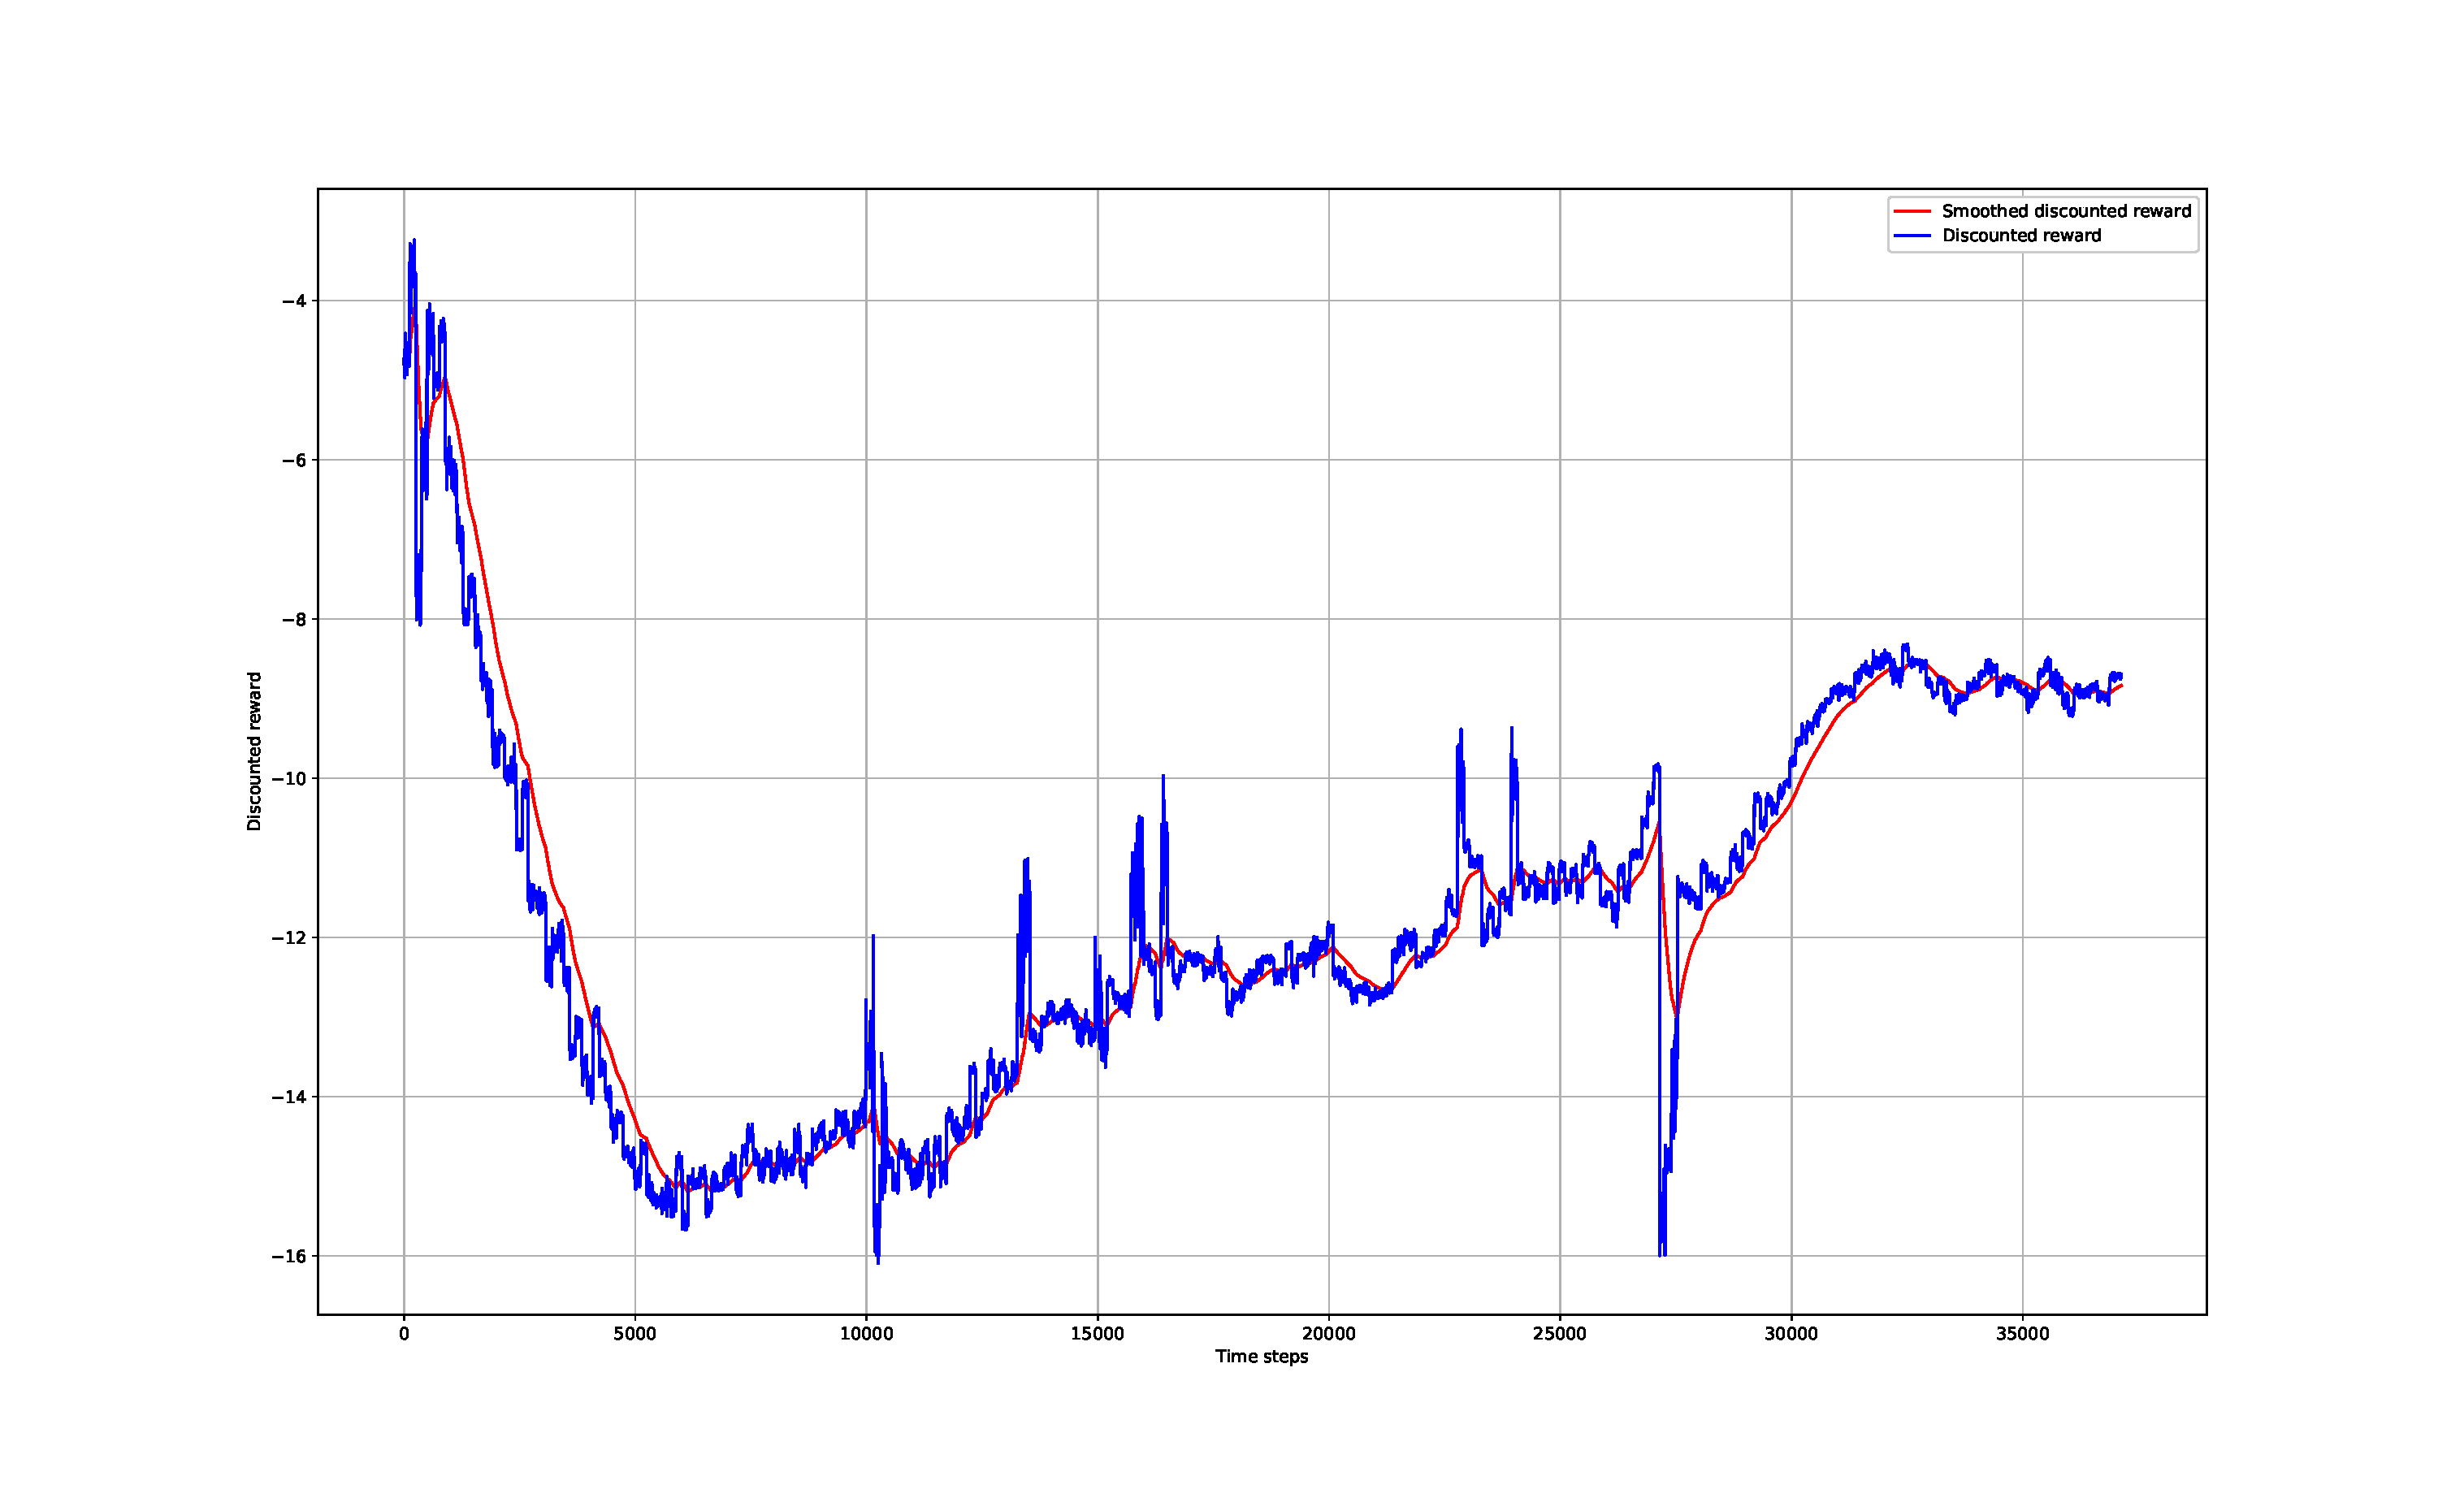
\includegraphics[scale=0.2]{Images/ppo2_1.eps}
	\caption{Learning curve of the PPO2 agent.  Discounted reward for the first 37500 time steps using default hyperparameters and negative normalized euclidean distances as rewards. The sudden drops around $10000$ and $27000$ are due to the resuming of training.}
	\label{reward_dist}
\end{figure}

While the curves on figure \ref{reward_dist} show the presence of learning, the resulting policy only showed a slight tendency to center the red dot on the webcam image. To improve these results, I decided to do two important modifications of the agent's implementation:

\begin{enumerate}
	\item Use the reward of equation \ref{gaussian_reward} to further penalize large distances;
	\item Reduce the bounds of the observation space to be in $[-1, 1]$.
\end{enumerate}

I then applied the same strategy as before, but for a higher number of time steps. At first, I let the agent learn statically, for $27000$ time steps i.e., with a fixed position of the Pi. Afterwards, I could already enjoy an agent that was able to center the red dot on the webcam under small motion of the Pi. Doing so for another $39000$ time steps during which the difficulty of the task increased led to a trained agent. This means that during these remaining time steps, I translated and rotated the Pi in every direction up to the point where it was "hardly" able to re-center the dot. This limit of feasibility increased throughout the training and finally allowed the agent to perform well even when the Pi was rotated by more than $90^{\circ}$. This learning process is shown on figure \ref{reward_dist2} where despite an increasing task complexity, the agent was able to maintain a slightly decreasing discounted reward in time. This time, the sudden drops in discounted reward are the result of both an increased task complexity (sudden rotation of the Pi) and/or the resuming of training. This agent constitutes the best result obtained in this project. The reader is invited to watch the \href{https://youtu.be/VGtoMPvjIwM}{demonstration video} to see how it performs in real life.

\begin{figure}[H]
	\centering
	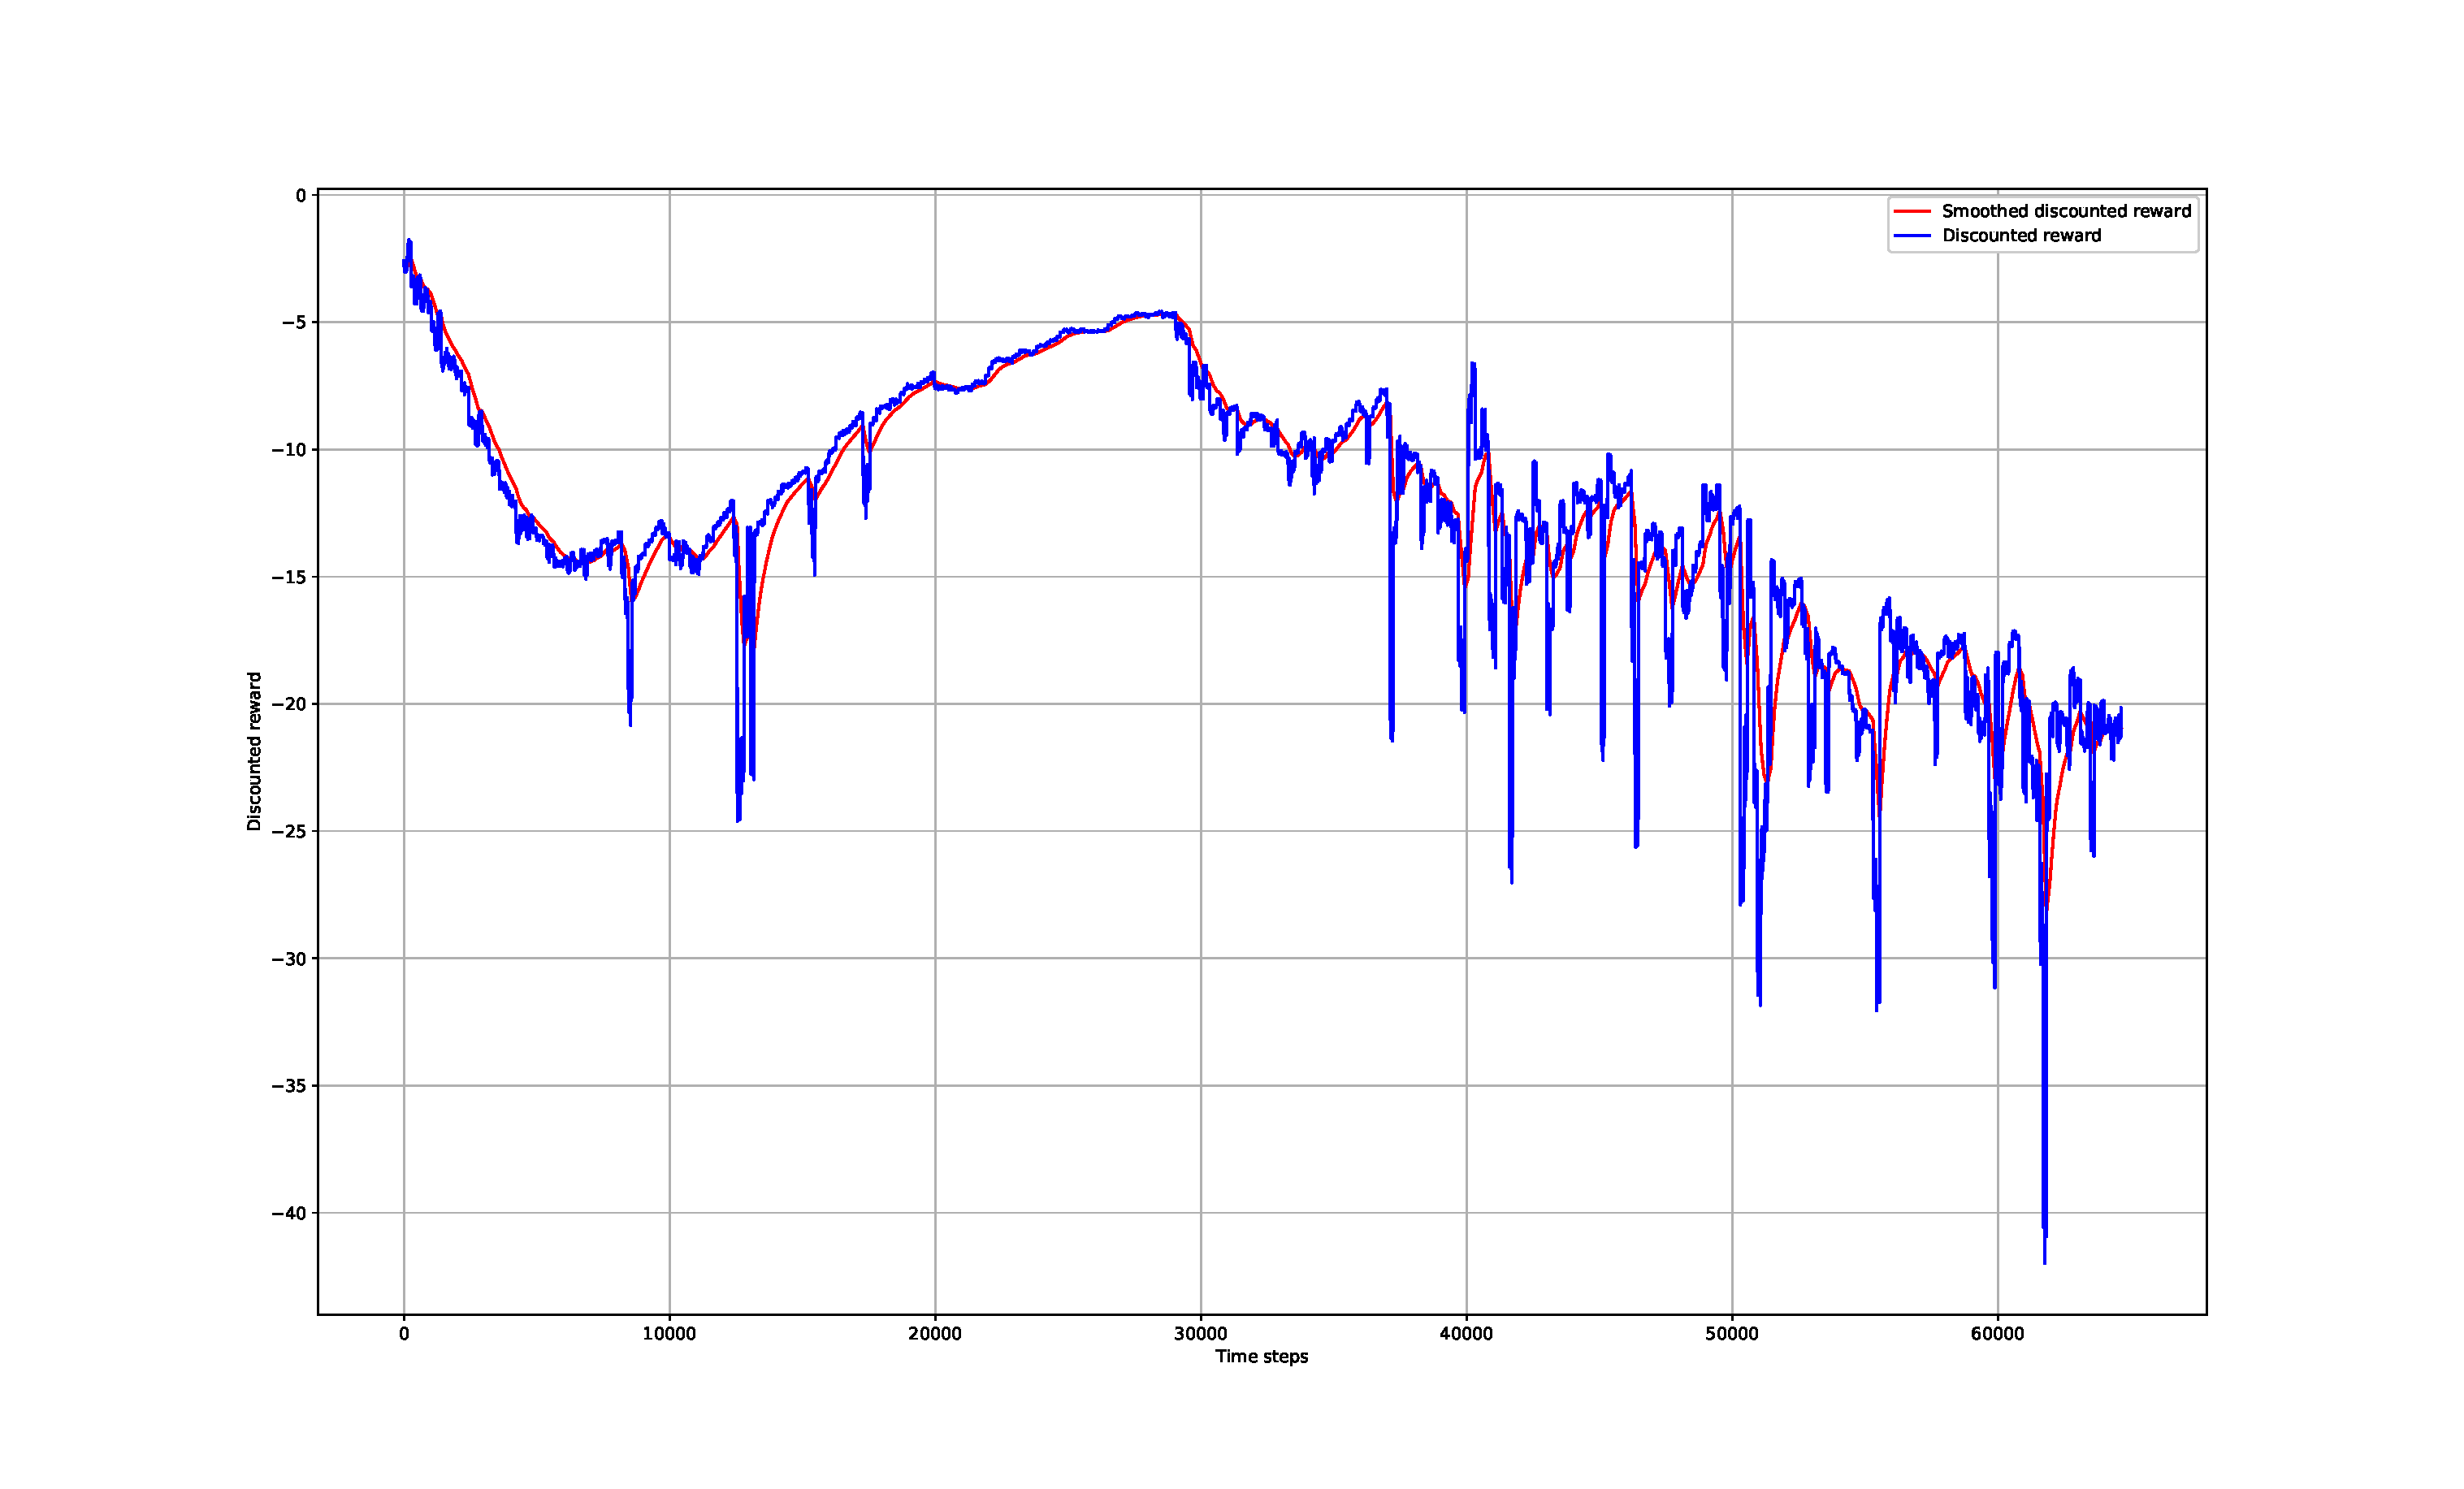
\includegraphics[scale=0.2]{Images/ppo2_2.eps}
	\caption{Learning curve of the PPO2 agent with rewards computed with equation \ref{gaussian_reward}. During the first $27000$ time steps, the Pi was hold fixed. The Pi was then rotated and translated during the remaining time steps with an increased task complexity, hence the slightly decreasing tendency of the learning curve.}
	\label{reward_dist2}
\end{figure}

\section{QDN}

A second and last agent was also implemented using the Deep-Q Network approach. In contrast to PPO2, this agent requires a careful tuning of its parameters in order to experience learning. The \texttt{\detokenize{config}} attribute of the agent class given in section \ref{agent} stores custom values for the DQN agent:

\begin{itemize}
	\item \texttt{\detokenize{learning_starts}}: timesteps used to fill experience buffer - set to 32;
	\item \texttt{\detokenize{target_network_update_freq}}: update the target network every - set to 100;
	\item \texttt{\detokenize{learning_rate}} : learning rate for adam optimizer - set to 0.001.
\end{itemize}

Despite tuning these hyperparameters and maintaining the Pi in a fixed position, the agent suffered from very slow learning, as shown on figure \ref{reward_dist3}. It is important to note that here we plot the reward obtained at every time step where one time step is the process of selecting an action and collecting the associated reward. In contrast, PPO2 considers a time steps to be a batch of 8 of such processes for which the discounted reward is the sum of the individual rewards obtained in that batch. The approximate number of $180000$ time steps in figure \ref{reward_dist3} would therefore correspond to $22500$ time steps in figure \ref{reward_dist2}. Note that again, drops in figure \ref{reward_dist3} indicate the resuming of training.

\begin{figure}[H]
	\centering
	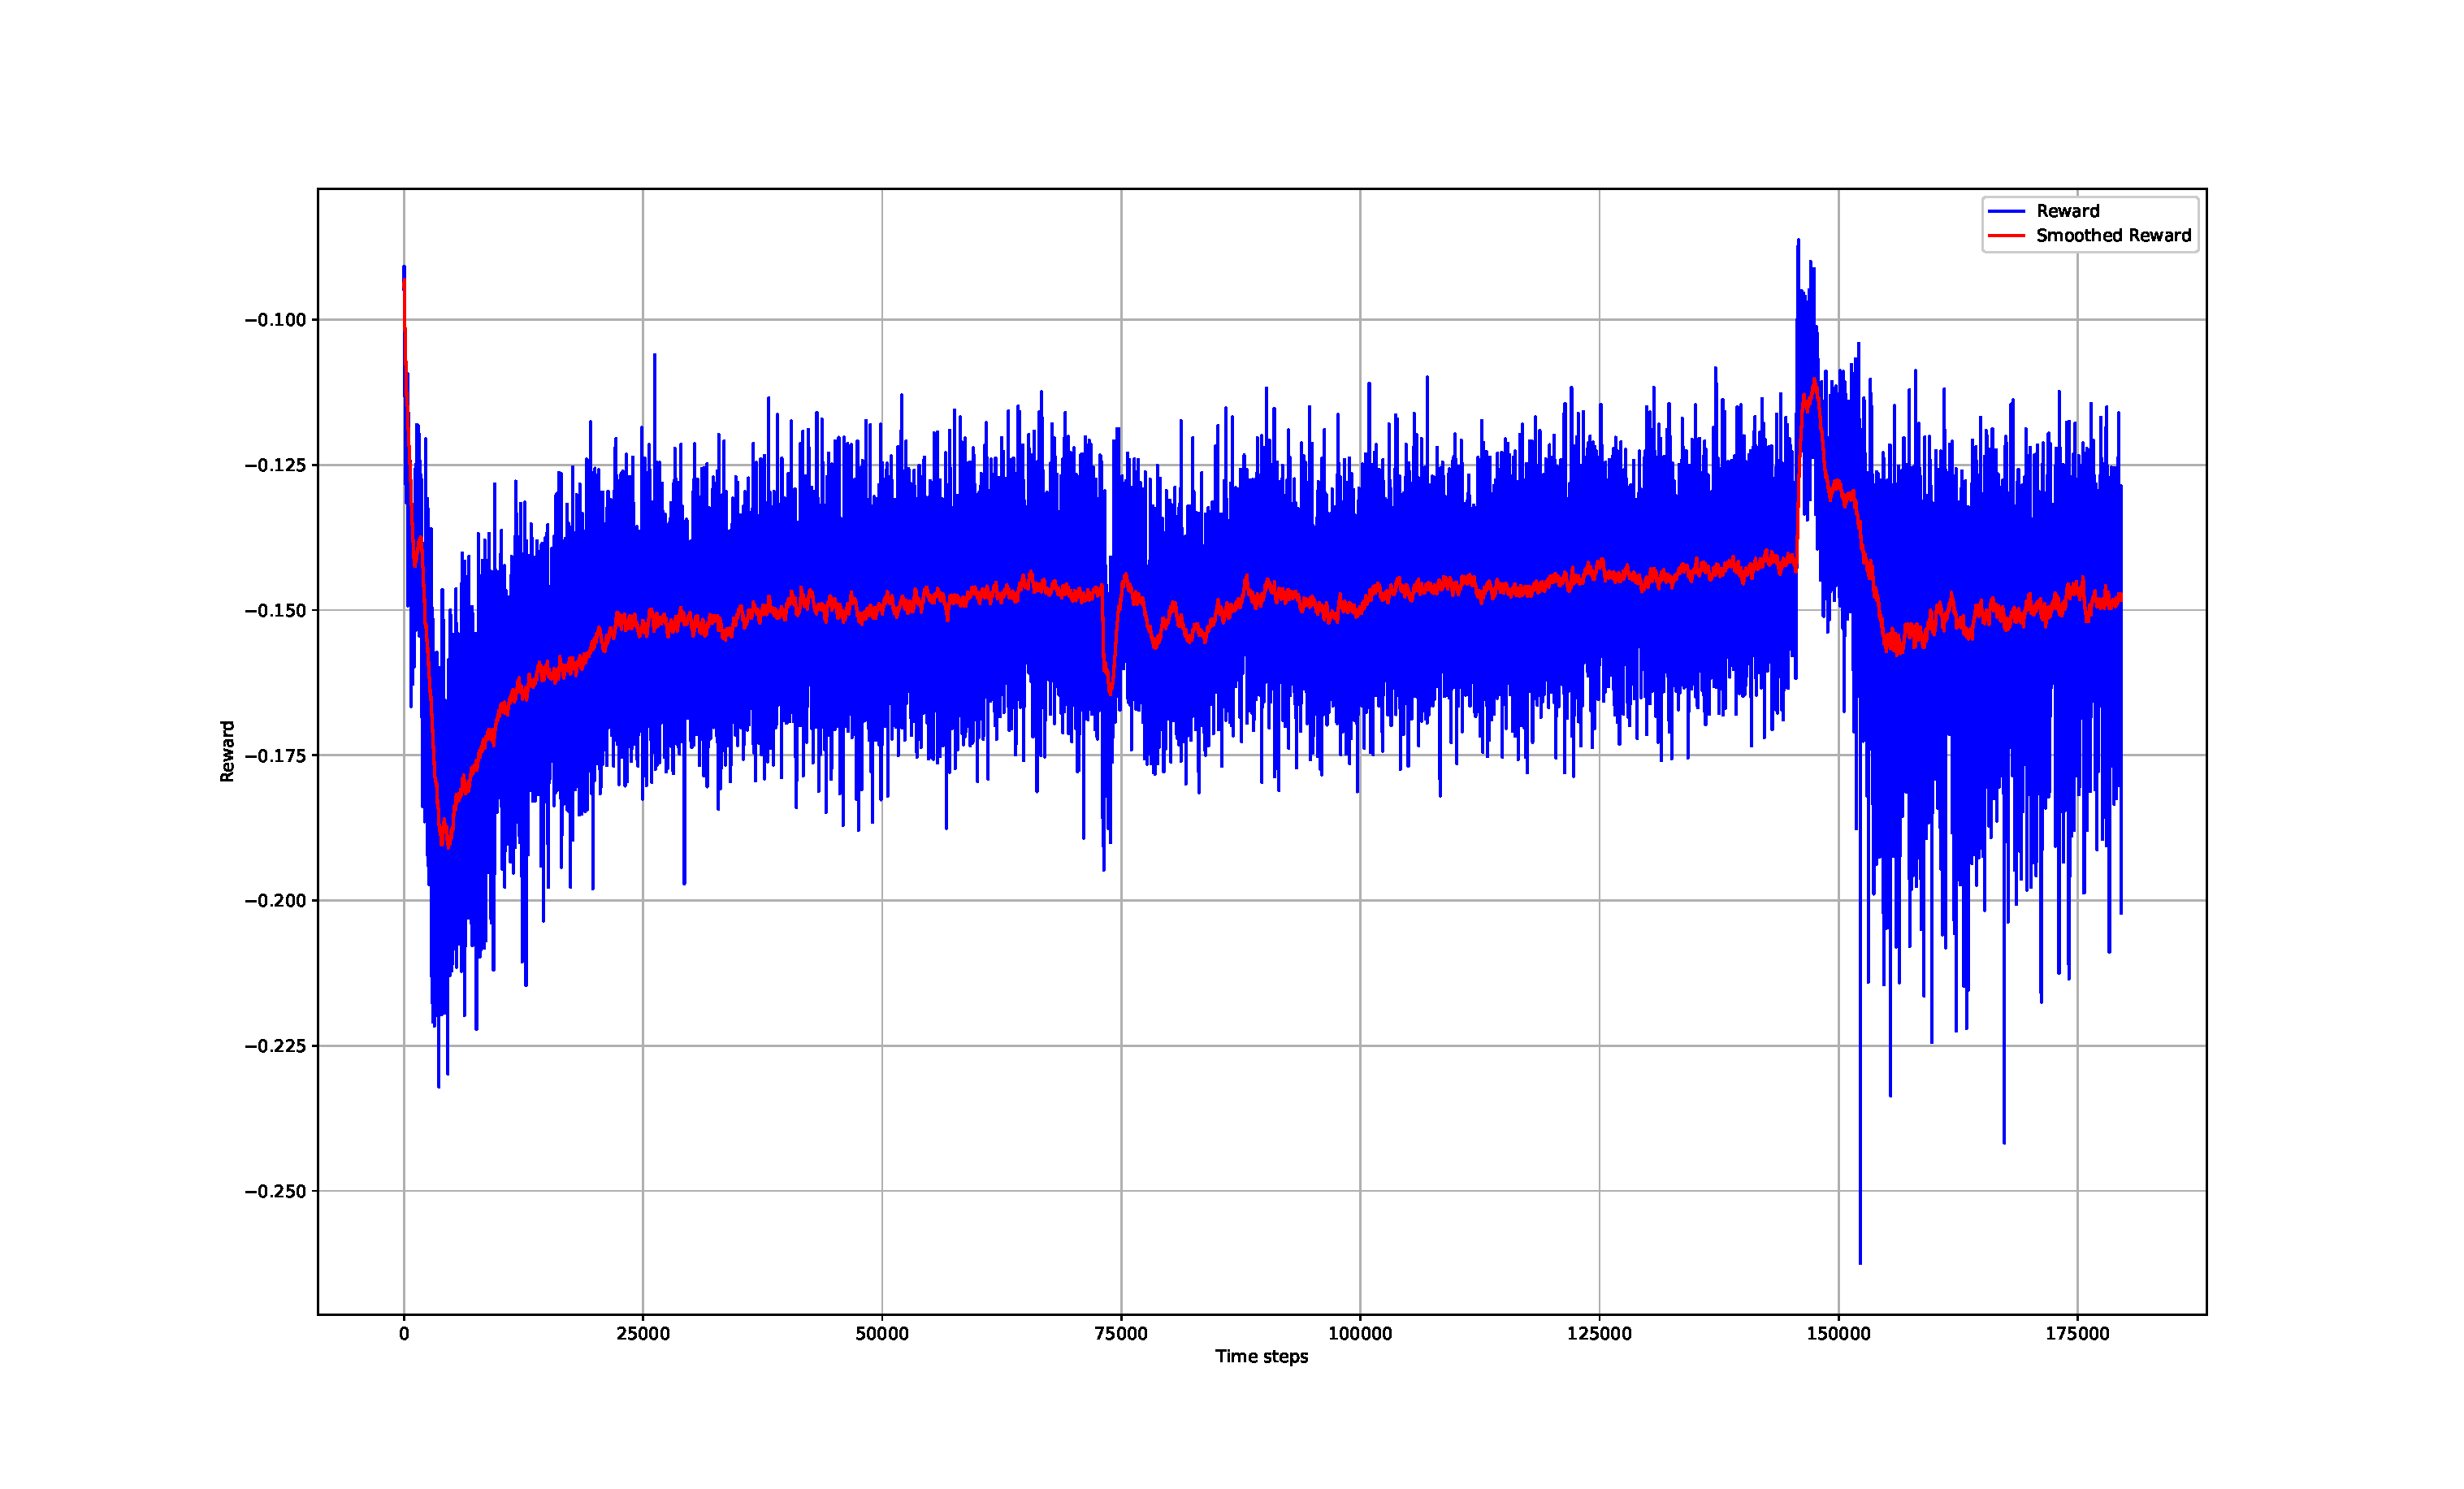
\includegraphics[scale=0.2]{Images/dqn.eps}
	\caption{Learning curve of the DQN agent. Despite tuning some of its hyperparameters and maintaining the Pi in a fixed position, the agent suffered from a very slow training.}
	\label{reward_dist3}
\end{figure}

As a result, the DQN agent does not perform as well as the PPO2 agent exposed in the previous section.  Further training and hyperparameter tuning could however produce better policies and is subject to future work. More importantly, this second agent displays the capacity of the underlying code to support other agents than PPO2 for which hyperparameters would need to be tuned wisely. Future efforts could therefore be spent on performing such tuning while benefiting from a robust training infrastructure that includes curriculum learning.

\section{Conclusion}

In this work, we presented an approach to solve the following problem: a person is allowed to hold a Raspberry Pi in front of a laptop's front camera. The goal is to train a RL agent so that the red light on the Pi's LED matrix is as close a possible to the webcam's image center despite the Pi being moved and/or rotated. To achieve such performance, we started by ensuring a communication between the agent on the PC side and the Pi on the server side using sockets. We used OpenCV to detect the position of the red dot on the webcam image. Results indicate that this position can be reliably computed even in the presence of daily light. After giving access to the Pi's acceleration and gyroscopic data to the agent, we created a custom gym environment in which the agent may learn. By carefully shaping the reward function, we were able to train a PPO2 agent that is capable of centering the red dot even if the Pi is being generously rotated and/or translated with respect to its centered position. In addition, we demonstrated the capacity of the underlying code to support other types of agents such as DQN that could potentially require a wise tuning of their hyperparameters. Future efforts could therefore be spent on training such agents on a large number of time steps thanks to the capacity of the code to provide curriculum learning across different runs.  Results of this work can be found in the \href{https://youtu.be/VGtoMPvjIwM}{demonstration video} as well as on the \href{https://github.com/avdhoeke/robotics}{github repository}.

\mychapter{3}{Appendix}

\section{Code on the Raspberry Pi}

\subsection{server.py}
\label{server_code}
\begin{pyverbatim}
import socket
from _thread import *
import pickle
import struct
from sense_hat import SenseHat
from rasp import Raspberry
import time

# Create server
s = socket.socket(socket.AF_INET, socket.SOCK_STREAM)
s.setsockopt(socket.SOL_SOCKET, socket.SO_REUSEADDR, 1)
s.bind(('0.0.0.0', 9395))
s.listen(10)
print("Waiting for a connection")

# Configure Sensehat
sense = SenseHat()
sense.clear()
rasp = Raspberry(sense)

def send(s, data):
    data = pickle.dumps(data)
    s.sendall(struct.pack('>i', len(data)))
    s.sendall(data)

def recv(s):
    data = s.recv(4, socket.MSG_WAITALL)
    data_len = struct.unpack('>i', data)[0]
    data = s.recv(data_len, socket.MSG_WAITALL)
    return pickle.loads(data)

def threaded_client(conn):
    # Declare global variables
    global sense

    while True:
        try:
            data = recv(conn)
            # Place our red dot at desired location
            if isinstance(data, list):
                rasp.place_dot(data)

            # Execute action required by RL agent
            else:
                rasp.move_led(data)

        except:
            pass
        
        # Send Gyroscope and accelerator data
        reply = rasp.acceleration + rasp.orientation
        send(conn, reply)

while True:
    # Accept client
    conn, addr = s.accept()
    print('Connected to:', addr)
    start_new_thread(threaded_client, (conn, ))
\end{pyverbatim}


\subsection{rasp.py}
\label{rasp_code}
\begin{pyverbatim}
import numpy as np


class Raspberry:

    def __init__(self, sense):
        self.sense = sense
        self.acceleration_ = None
        self.orientation_ = None
        self.led = [0, 0]

    @property
    def acceleration(self):
        acc = self.sense.get_accelerometer_raw()
        return [acc['x'], acc['y'], acc['z']]

    @property
    def orientation(self):
        gyro = self.sense.get_gyroscope_raw()
        return [gyro['x'], gyro['y'], gyro['z']]

    def place_dot(self, pos: np.ndarray) -> None:
        self.sense.clear()
        pos = pos[0]
        print("Resettting pixel ({}, {})".format(pos[0], pos[1]))
        self.sense.set_pixel(pos[0], pos[1], (255, 0, 0))

    def move_led(self, action: int) -> None:

        self.sense.clear()
        x, y = self.led[0], self.led[1]

        if action == 0:  # Move to the right
            self.led[0] = x-1 if x>0 else x

        if action == 1:  # Move the the left
            self.led[0] = x+1 if x<7 else x

        if action == 2:  # Move upwards
            self.led[1] = y-1 if y>0 else y

        if action == 3:  # Move down
            self.led[1] = y+1 if y<7 else y
        
        if action == 4:  # Stay at the same position
            self.led[0], self.led[1] = x, y
        
        self.sense.set_pixel(self.led[0], self.led[1], (255, 0, 0))

\end{pyverbatim}

\section{Code on the PC}
\subsection{network.py}
\label{pc_code}

\begin{pyverbatim}
import socket
import pickle
import struct


class Network:

    def __init__(self):
        self.client = socket.socket(socket.AF_INET, socket.SOCK_STREAM)
        self.client.setsockopt(socket.IPPROTO_TCP, socket.TCP_NODELAY, 1)
        self.host = "192.168.1.40"
        self.port = 9395
        self.addr = (self.host, self.port)
        self.client.connect(self.addr)

    def send(self, data) -> None:
        data = pickle.dumps(data)
        self.client.sendall(struct.pack('>i', len(data)))
        self.client.sendall(data)

    def recv(self) -> list:
        data = self.client.recv(4, socket.MSG_WAITALL)
        data_len = struct.unpack('>i', data)[0]
        data = self.client.recv(data_len, socket.MSG_WAITALL)
        return pickle.loads(data)

\end{pyverbatim}

\section{OpenCV code}

\subsection{calibrate.py}
\label{calibrate}

\begin{pyverbatim}
import cv2
import numpy as np


def run():
    while True:

        def nothing(x):
            pass

        # Create a window
        cv2.namedWindow('image')

        # create trackbars for color change
        cv2.createTrackbar('HMin', 'image', 0, 179, nothing)
        cv2.createTrackbar('SMin', 'image', 0, 255, nothing)
        cv2.createTrackbar('VMin', 'image', 0, 255, nothing)
        cv2.createTrackbar('HMax', 'image', 0, 179, nothing)
        cv2.createTrackbar('SMax', 'image', 0, 255, nothing)
        cv2.createTrackbar('VMax', 'image', 0, 255, nothing)

        # Set default value for MAX HSV trackbars.
        cv2.setTrackbarPos('HMax', 'image', 179)
        cv2.setTrackbarPos('SMax', 'image', 255)
        cv2.setTrackbarPos('VMax', 'image', 255)

        # Initialize to check if HSV min/max value changes
        hMin = sMin = vMin = hMax = sMax = vMax = 0
        phMin = psMin = pvMin = phMax = psMax = pvMax = 0

        # OpenCV function
        WINDOW_NAME = "Calibration of filter"
        cv2.namedWindow(WINDOW_NAME)
        vc = cv2.VideoCapture(0)  # Initialize the default camera

        try:
            if vc.isOpened():  # try to get the first frame
                (readSuccessful, frame) = vc.read()
            else:
                raise (Exception("failed to open camera."))

            while readSuccessful:

                # get current positions of all trackbars
                hMin = cv2.getTrackbarPos('HMin', 'image')
                sMin = cv2.getTrackbarPos('SMin', 'image')
                vMin = cv2.getTrackbarPos('VMin', 'image')

                hMax = cv2.getTrackbarPos('HMax', 'image')
                sMax = cv2.getTrackbarPos('SMax', 'image')
                vMax = cv2.getTrackbarPos('VMax', 'image')

                # Set minimum and max HSV values to display
                lower = np.array([hMin, sMin, vMin])
                upper = np.array([hMax, sMax, vMax])

                # Create HSV Image and threshold into a range.
                hsv = cv2.cvtColor(frame, cv2.COLOR_BGR2HSV)
                mask = cv2.inRange(hsv, lower, upper)
                output = cv2.bitwise_and(frame, frame, mask=mask)

                # Print if there is a change in HSV value
                if ((phMin != hMin) | (psMin != sMin) | (pvMin != vMin) |\
                 (phMax != hMax) | (psMax != sMax) | (pvMax != vMax)):
                    print("(hMin = %d , sMin = %d, vMin = %d), 
                               (hMax = %d , sMax = %d, vMax = %d)"
                                % (hMin, sMin, vMin, hMax, sMax, vMax))
                    phMin = hMin
                    psMin = sMin
                    pvMin = vMin
                    phMax = hMax
                    psMax = sMax
                    pvMax = vMax

                # Display output image
                cv2.imshow('image', output)
                #############################

                # Set refreshing time
                key = cv2.waitKey(10)
                if key == 27:  # exit on ESC
                    break
                # Get Image from camera
                readSuccessful, frame = vc.read()
        finally:
            vc.release()  # close the camera
            cv2.destroyWindow(WINDOW_NAME)  # close the window


run()

\end{pyverbatim}

\subsection{processing.py}
\label{processing}
\begin{pyverbatim}
import cv2
import numpy as np
from typing import *


def get_red_dot(env, display_images: bool) -> None:

    # Get attributes of environment instance
    frame = env.frame

    # Process the input image from webcam
    total, red, final = filter_image(frame)

    # Place our red dot on image
    x, y, image = compute_red_dot(final, frame)

    if display_images:
        # Display the resulting filtered images
        cv2.imshow('Image filtered with mask', total)
        cv2.imshow('Filtered image with red dominance', red)
        cv2.imshow('Filtered image with binary threshold', final)

    # Display final image with red square on it
    cv2.imshow('Original image with red square', image)

    # Set new square location
    env.square = [x, y]


def filter_image(frame: np.ndarray) -> Tuple[np.ndarray, np.ndarray, np.ndarray]:

    # Convert BGR to HSV format
    _ = cv2.cvtColor(frame, cv2.COLOR_BGR2HSV)

    # lower boundary RED color range values; Hue (0 - 10)
    lower1 = np.array([0, 0, 217])
    upper1 = np.array([10, 255, 255])

    # upper boundary RED color range values; Hue (90 - 180)
    lower2 = np.array([90, 0, 230])
    upper2 = np.array([179, 255, 255])

    # Apply filters defined previously
    lower_mask = cv2.inRange(_, lower1, upper1)
    upper_mask = cv2.inRange(_, lower2, upper2)

    full_mask = lower_mask + upper_mask

    total = cv2.bitwise_and(frame, frame, mask=full_mask)

    # Additional Red color filter
    low_red = np.array([10, 0, 0])
    high_red = np.array([180, 150, 255])
    red_mask = cv2.inRange(total, low_red, high_red)
    red = cv2.bitwise_and(frame, frame, mask=red_mask)

    # Threshold the resulting image
    h, s, v = cv2.split(red)
    ret, final = cv2.threshold(v, 150, 255, cv2.THRESH_BINARY)

    return total, red, final


def compute_red_dot(final: np.ndarray, frame: np.ndarray) -> \
Tuple[Union[None, float], Union[None, float], np.ndarray]:

    # Dilatation of filtered image
    dilatation = cv2.dilate(final, np.ones((3, 3)))
    retval,labels,stats,centroids = cv2.connectedComponentsWithStats(dilatation)

    # Compute position of biggest red area
    x, y = None, None
    max_area = None

    for stat, center in zip(stats[1:], centroids[1:]):
        area = stat[4]

        if (max_area is None) or (area > max_area):
            x, y = center
            max_area = area

    image = np.copy(frame)

    # Put blue square at the center of the image
    image[360 - 10:360 + 10, 640 - 10:640 + 10, :] = (255, 100, 100)

    if x is not None and y is not None:
        x, y = int(x), int(y)
        image[y - 10:y + 10, x - 10:x + 10, :] = (100, 100, 255)
        return float(x), float(y), image

    else:
        return x, y, image

\end{pyverbatim}

\section{RL framework}

\subsection{environment.py}
\label{environment}
\begin{pyverbatim}

from abc import ABC
import gym
from src import Network
from . processing import *
import time


class RaspEnv(gym.Env, ABC):
    def __init__(self):
        # The Discrete space allows a fixed range of non-negative numbers
        self.action_space = gym.spaces.Discrete(4)
        # Shape of observation space
        self.observation_shape = (8,)
        # The Box space represents an n-dimensional box
        self.observation_space = gym.spaces.Box(
                 shape=self.observation_shape,
                 low=np.array([-1.0, -1.0, -1.0, -1.0, -1.0, -1.0, -1.0, -1.0]),
                 high=np.array([1.0, 1.0, 1.0, 1.0, 1.0, 1.0, 1.0, 1.0]),
                 dtype=np.float64)
        # Coordinates of red dot on pc screen
        self.square_ = [0.0, 0.0]
        # Link with our Raspberry to receive observations
        self.network = Network()
        # Record video from webcam number 0
        self.cap = cv2.VideoCapture(0)
        # Monitor the existence of a red dot
        self.trainable = True

    @property
    def frame(self):
        # try to get the first frame
        if self.cap.isOpened():
            # frame has shape (720, 1280, 3)
            readSuccessful, frame = self.cap.read()
        else:
            raise (Exception("failed to open camera."))
        return frame

    @property
    def square(self):
        get_red_dot(self, False)
        return self.square_

    @square.setter
    def square(self, s: list):
        self.square_ = s
        if s[0] is None and s[1] is None:
            print("Lost position of red dot !")
            self.trainable = False
        else:
            self.trainable = True

    def step(self, action: int) -> Tuple[np.ndarray, float, bool, dict]:

        # The default resulting outcome is: keep training !
        done = False

        # Send action to Raspberry Pi
        self.network.send(action)

        # Let a small time laps to PC before fetching the env's response
        time.sleep(0.2)

        # Get ax, ay, az, gx, gy, gz from Raspberry Pi
        obs = self.network.recv()

        # Update location of red dot on PC screen
        get_red_dot(env=self, display_images=False)

        # Prevent agent from learning if red dot disappears
        if not self.trainable:
            obs += [e for e in [0.0, 0.0]]
            obs = np.asarray(obs)
            reward = np.random.rand(1)[0]
            done = True

        else:
            # normalize the position of the dot
            x, y = (self.square_[0] - 640) / 640, (self.square_[1] - 360) / 360

            # Add red dot position to observation
            obs.append(x)
            obs.append(y)
            obs = np.asarray(obs)

            # Compute reward from red dot position
            reward = self.compute_reward(x, y)

        # To allow cap to be used in a loop
        cv2.waitKey(10)

        return obs, reward, done, {}

    def compute_reward(self, x: float, y: float) -> float:

        # Compute euclidean distance
        # distance = -np.sqrt(x ** 2 + y ** 2)

        # Compute distance with "gaussian kernel"
        distance = 1 - np.exp(np.sqrt(x ** 2 + y ** 2))

        return distance

    def reset(self) -> np.ndarray:

        # Reset red dot position
        pos = np.random.randint(0, 8, 2)

        # Put red dot at random initial locations
        self.network.send([pos])

        # Get Raspberry acceleration and gyroscopic data
        obs = self.network.recv()

        obs += [e for e in [0.0, 0.0]]
        obs = np.asarray(obs)

        return np.zeros(8)

    def render(self, mode='human'):
        pass

\end{pyverbatim}

\subsection{agent.py}
\label{agent}
\begin{pyverbatim}
from . processing import *
from .environment import RaspEnv
import tensorflow as tf
import warnings
import abc
import os
from stable_baselines.common.env_checker import check_env
from stable_baselines.common.callbacks import StopTrainingOnRewardThreshold,  \
EvalCallback, CallbackList, CheckpointCallback
from stable_baselines.common.vec_env import DummyVecEnv
tf.compat.v1.logging.set_verbosity(tf.compat.v1.logging.ERROR)
warnings.filterwarnings("ignore", category=UserWarning)


class Agent:

    def __init__(self, model: abc.ABCMeta):
        # Define new environment
        self.env = RaspEnv()
        # Check if environment is ok
        check_env(self.env)
        # Define empty model
        self.model = model
        # Configure model hyperparameters
        self.config = {'learning_starts': 32, 
                       'target_network_update_freq': 100, 
                       'learning_rate': 0.001}

    def load_model(self, tensorboard_log: str) -> None:

        # Get path of latest model
        path = os.getcwd()
        os.chdir(os.getcwd() + '/model_checkpoints')

        # Process all the files in the folder
        files = [x for x in os.listdir() if x.endswith(".zip")]
        num = []
        for file in files:
            num.append([int(x) for x in file.split('_') if x.isdigit()][0])
        filename = "rl_model_" + str(max(num)) + "_steps.zip"

        # Load most recent model
        self.model = self.model.load(load_path=filename,
                                     env=DummyVecEnv([lambda: self.env]),
                                     tensorboard_log=tensorboard_log,
                                     **self.config)
        print("Successfully loaded the previous model: " + filename)

        # Return to root path
        os.chdir(path)

    def create_model(self, tensorboard_log: str) -> None:

        # Vector-encode our new environment
        env = DummyVecEnv([lambda: self.env])

        # Create new model
        self.model = self.model('MlpPolicy', 
                                 env, verbose=1,
                                 tensorboard_log=tensorboard_log,
                                 **self.config)
        print(type(self.model))
        print("Successfully created new model")

    def train(self, tensorboard_log: str) -> None:

        try:
            self.load_model(tensorboard_log=tensorboard_log)

        except:
            self.create_model(tensorboard_log=tensorboard_log)

        # Stop training if reward gets close to zero
        callback_on_best = StopTrainingOnRewardThreshold(reward_threshold=-0.1, 
                                                         verbose=1)
                                                                                           
        eval_callback = EvalCallback(self.env, 
                                     callback_on_new_best=callback_on_best, 
                                     verbose=1)

        # Save model at regular time intervals
        checkpoint_callback = CheckpointCallback(save_freq=1000, 
                                                 save_path='./model_checkpoints/')

        # Chain callbacks together
        callback = CallbackList([eval_callback, checkpoint_callback])

        # Train model
        self.model.learn(total_timesteps=int(1e10), 
                           callback=callback, 
                           tb_log_name="run")

        # Save trained model
        print("Training is finished!")

    def evaluate(self, tensorboard_log: str) -> None:

        self.create_model(tensorboard_log)
        obs = self.env.reset()

        while True:

            # Compute action based on previous observation
            action, _states = self.model.predict(obs, deterministic=True)
            # Compute observation and reward from the action that was sent
            obs, rewards, done, info = self.env.step(action)
            if done:
                obs = self.env.reset()
                
\end{pyverbatim}

